\documentclass{beamer}
%\documentclass[noteonly]{beamer}

\usepackage[OT4]{fontenc}
\usepackage[utf8]{inputenc}
\usepackage[polish]{babel}

\usepackage{listings}

\usepackage{color}
\usepackage{xcolor}
\usepackage{beamerthemesplit}
%\usetheme{Berkeley}
\usetheme{Madrid}
%\usecolortheme{crane}

\xdefinecolor{nvidia}{rgb}{0.463,0.725,0.0}

\setbeamercolor{alerted text}{fg=red}
\setbeamercolor{example text}{fg=orange}
\setbeamercolor{structure}{fg=nvidia,bg=black}
\setbeamercolor*{palette primary}{fg=nvidia,bg=black}
\setbeamercolor*{palette secondary}{fg=nvidia,bg=black}
\setbeamercolor*{palette tertiary}{bg=nvidia,fg=gray!50!black}
\setbeamercolor*{palette quaternary}{fg=nvidia,bg=gray!20!black}

\setbeamercolor*{sidebar}{fg=nvidia,bg=black!75!white}

\setbeamercolor*{palette sidebar primary}{fg=nvidia!10!black}
\setbeamercolor*{palette sidebar secondary}{fg=white}
\setbeamercolor*{palette sidebar tertiary}{fg=nvidia!50!black}
\setbeamercolor*{palette sidebar quaternary}{fg=gray!10!black}

\setbeamercolor*{titlelike}{parent=palette primary}
\setbeamercolor{frametitle}{bg=black}
\setbeamercolor{frametitle right}{bg=black}

\setbeamercolor*{separation line}{}
\setbeamercolor*{fine separation line}{}

\setbeamercolor{block title}{use=structure,fg=nvidia,bg=black}
\setbeamercolor{block title alerted}{use=alerted text,fg=red,bg=black}
\setbeamercolor{block title example}{use=example text,fg=orange,bg=black}

\setbeamercolor{block body}{parent=normal text,use=block title,bg=block title.bg!10!bg}
\setbeamercolor{block body alerted}{parent=normal text,use=block title alerted,bg=block title alerted.bg!10!bg}
\setbeamercolor{block body example}{parent=normal text,use=block title example,bg=block title example.bg!10!bg}

\usenavigationsymbolstemplate{}
\usefonttheme{professionalfonts}

\lstset{ %
language=XML,                % choose the language of the code
basicstyle=\scriptsize,       % the size of the fonts that are used for the code
keywordstyle={\color{nvidia}\textbf},
commentstyle={\color{gray}\textit},
backgroundcolor=\color{white},  % choose the background color. You must add \usepackage{color}
showspaces=false,               % show spaces adding particular underscores
showstringspaces=false,         % underline spaces within strings
showtabs=false,                 % show tabs within strings adding particular underscores
frame=single,	                % adds a frame around the code
tabsize=4,	                % sets default tabsize to 2 spaces
captionpos=b,                   % sets the caption-position to bottom
breaklines=true,                % sets automatic line breaking
breakatwhitespace=false,        % sets if automatic breaks should only happen at whitespace
title=\lstname,                 % show the filename of files included with \lstinputlisting; also try caption instead of title
escapeinside={\%*}{*)},          % if you want to add a comment within your code
}

%\AtBeginSection{
%	\begin{frame}
%		\begin{center}
%			\structure{\Huge \insertsection}
%		\end{center}
%	\end{frame}
%}


%\AtBeginSubsection{
%	\begin{frame}
%		\begin{center}
%			\structure{\LARGE \insertsubsection}
%		\end{center}
%	\end{frame}
%}

\title[Data reliability and integrity]{Managing data reliability and integrity in federated cloud storage}
\author[Krzysztof Styrc ACC CYFRONET]{
Krzysztof Styrc ACC CYFRONET\\
\noindent
kstyrc@gmail.com
}
\date[]{
Promotor:\\
\noindent
dr inż. Marian Bubak
}

\begin{document}

\frame{\titlepage}

\begin{frame}
\begin{block}{\textbf{Data validation is a well explored area:}}
\begin{itemize}
	\item hash functions (MD5, SHA-1, etc),
	\item message authentication codes (MAC),
	\item error correcting codes (ECC).
\end{itemize}
\end{block}
\begin{exampleblock}{\textbf{However, emerging popularity of cloud storage services carry on new challenges. Storing vast amounts of data on external resources will probably result in network ineffciencies when calculating the whole file checksums. Proof of Retrievability (POR) algorithms try to solve this performance issues.}}
\begin{figure}
\centering
\includegraphics[scale=0.04]{por.png}
\end{figure}
\end{exampleblock}
\end{frame}

\begin{frame}
\begin{block}{\textbf{Long-term persistence of medical data sets requires reliability and integrity mechanisms to be built on top of Cloud storage. DRI is designed to fullfill these requirements by performing the following tasks:}}
\begin{itemize}
	\item periodic and request-driven integrity checks on data sets,
	\item facilitating storage of multiple copies of data on various Cloud platforms,
	\item tracking the history and origin of binary data sets.
\end{itemize}
\end{block}
\begin{exampleblock}{\textbf{Datasets validation:}}
\begin{itemize}
	\item availability of each dataset at its (multiple) locations,
	\item the integrity of each dataset's file (checksum-based).
\end{itemize}
\end{exampleblock}
\end{frame}

\begin{frame}
\begin{block}{\textbf{DRI Service:}}
\begin{itemize}
	\item stateless REST WebService,
	\item built on top of AIR registry and multiple of cloud storage,
	\item self-running daemon (periodic checks) and API access,
\end{itemize}
\end{block}
\begin{figure}
\centering
\includegraphics[scale=0.28]{schemat.pdf}
\end{figure}
\end{frame}

\begin{frame}
\begin{block}{\textbf{Current functionalities:}}
\begin{itemize}
	\item supported requests: dataset validation and adding dataset under management (computing its checksums),
	\item integrity checks based on SHA-256 of the first 1KB of a file -- for fast testing on large datasets,
	\item asynchronous operations added to queue of a simple scheduler,
	\item report notifications (validation success/failure or finished adding dataset under management) as emails,
\end{itemize}
\end{block}
\begin{exampleblock}{\textbf{Current REST API:}}
\begin{itemize}
	\item \textbf{\textit{add\_dataset\_under\_management/\{datasetID\}}} -- asynchronously computing dataset's files checksums and notify by email,
	\item \textbf{\textit{validate\_dataset/\{datasetID\}}} -- asynchronously validate dataset and notify by email.
\end{itemize}
\end{exampleblock}
\end{frame}

\begin{frame}
\begin{block}{\textbf{On-going work:}}
\begin{itemize}
	\item further integration with AIR registry,
	\item support for S3 storage besides Swift,
	\item efficient validation algorithm research,
	\item periodic validation based on scheduler,
\end{itemize}
\end{block}
\begin{exampleblock}{\textbf{Efficient validation -- DRI challenge:}}
\begin{itemize}
	\item the number and size of stored datasets can be vast,
	\item existing Cloud storage API's (Swift, S3) flexibility is limited,
	\item serving data -- primary service , validation -- secondary service,
	\item need for efficient and effective validation algorithm.
\end{itemize}
\end{exampleblock}
\end{frame}

%\section*{Bibliografia}
%\nocite{*}
%\bibliographystyle{plplain}
%\bibliography{biblio}


\end{document}
